\documentclass{llncs}
\usepackage{graphicx}
\usepackage[caption=false]{subfig}
\usepackage[dvipsnames]{xcolor}
\usepackage{amssymb}
\usepackage{amsmath}
\usepackage{todonotes}

\title{Old or Heavy?\\Decaying Gracefully with Age/Weight Shapes.}
\titlerunning{Dynamic Strategy Priority}
\authorrunning{Reger \and Rawson}
\author{Michael Rawson \and Giles Reger}
\institute{University of Manchester, Manchester, UK}

\newcommand{\tick}{\ding{52}}

%
% Pieces from the old manual that are still useful for the future.
%

\newcommand{\old}[1]{}
%\newcommand{\old}[1]{{\color{red}#1}}

%
% Re-definitions of LaTeX commands
%

\renewcommand{\floatpagefraction}{0.9}

% part (to produce a correct entry in TOC
%\makeatletter
%\def\@part[#1]#2{%
%    \ifnum \c@secnumdepth >-2\relax
%      \refstepcounter{part}%
%%      \addcontentsline{toc}{part}{\thepart\hspace{1em}#1}%
%      \addcontentsline{toc}{part}{#1}%
%    \else
%      \addcontentsline{toc}{part}{#1}%
%    \fi
%    \markboth{}{}%
%    {\centering
%     \interlinepenalty \@M
%     \normalfont
%     \ifnum \c@secnumdepth >-2\relax
%       \huge\bfseries \partname~\thepart
%       \par
%       \vskip 20\p@
%     \fi
%     \Huge \bfseries #2\par}%
%    \@endpart}
%\makeatother

\newcommand{\fullref}[1]{\ref{#1} on page~\pageref{#1}}

%
%
%   the beast
%
%

\newcommand{\Vampire}{\textsc{Vampire}}
\newcommand{\VWP}{\url{http://www.vprover.org}}

%
%   general
%

%\newcommand{\eqref}[1]{(\ref{#1})}
\newcommand{\setof}[1]{\{#1\}}
\newcommand{\xone}[2]{#1_1,\ldots,#1_{#2}}
\newcommand{\xzero}[2]{#1_0,\ldots,#1_{#2}}
\newcommand{\QEDsymbol}{\text{\ding{111}}}
\newcommand{\QED}{\hfill\QEDsymbol}
\newcommand{\bydef}{\stackrel{\text{def}}{=}}       % by definition


%
%
%     Indexing
%
%

\newcommand{\dindex}[1]{\index{#1|textbf}}
\newcommand{\D}[1]{\DI{#1}{#1}}                       % emphasize + boldface index
\newcommand{\DI}[2]{\emph{#1}\dindex{#2}}             % emphasize + boldface index
\newcommand{\DII}[3]{\emph{#1}\dindex{#2}\dindex{#3}} % emphasize + 2 boldface indices
\newcommand{\DIII}[4]{\emph{#1}\dindex{#2}\dindex{#3}\dindex{#4}} % emphasize + 3 boldface indices
\newcommand{\DIIII}[5]{\emph{#1}\dindex{#2}\dindex{#3}\dindex{#4}\dindex{#5}} % emphasize + 4 boldface indices
\newcommand{\E}[1]{\EI{#1}{#1}}                       % emphasize + index
\newcommand{\EI}[2]{\emph{#1}\index{#2}}     % emphasize + index
\newcommand{\EII}[3]{\emph{#1}\index{#2}\index{#3}} % emphasize + 2 indices

%
%
% Algorithms
%
%

\newcommand{\inc}{~~~~\= \+ \kill}    % used in algorithms
\newcommand{\dec}{\- \kill}         % used in algorithms

\newcommand{\reserved}[1]{\textbf{\underline{#1}}} % reserved words in algorithms
\newcommand{\semicol}{;}                  % semicolon in algorithms
\newcommand{\assign}{\texttt{:=}}                  % assignment in algorithms
\newcommand{\commentinalg}[1]{\texttt{(* #1 *)}}         % comment in algorithms
\newcommand{\PROCEDURE}{\reserved{procedure}}
\newcommand{\SUBPROCEDURE}{\reserved{subprocedure}}
\newcommand{\PARAMETERS}{\reserved{parameters}}
\newcommand{\INPUT}{\reserved{input}}
\newcommand{\OUTPUT}{\reserved{output}}
\newcommand{\IF}{\reserved{if}}
\newcommand{\VAR}{\reserved{var}}
\newcommand{\CASE}{\reserved{case}}
\newcommand{\OF}{\reserved{of}}
\newcommand{\DO}{\reserved{do}}
\newcommand{\OD}{\reserved{od}}
\newcommand{\THEN}{\reserved{then}}
\newcommand{\ELSE}{\reserved{else}}
\newcommand{\WHILE}{\reserved{while}}
\newcommand{\BEGIN}{\reserved{begin}}
\newcommand{\END}{\reserved{end}}
\newcommand{\LET}{\reserved{let}}
\newcommand{\FORALL}{\reserved{forall}}
\newcommand{\ASS}{\texttt{ := }}
\newcommand{\RETURN}{\reserved{return}}
\newcommand{\REPEAT}{\reserved{repeat}}
\newcommand{\LOOP}{\reserved{loop}}
\newcommand{\FOREACH}{\reserved{foreach}}

% saturation

\newcommand{\supS}{\mathrm{Sup}}
\newcommand{\isS}{\mathbb{I}}
\newcommand{\deleted}{\cancel}
\newcommand{\Mark}{\ensuremath{\checkmark}}
\newcommand{\Active}{\ensuremath{\mathit{active}}}
\newcommand{\DeActive}{\mathit{deactivated}}
\newcommand{\Kept}{\mathit{kept}}
\newcommand{\Passive}{\ensuremath{\mathit{passive}}}
\newcommand{\Init}{\mathit{init}}
\newcommand{\New}{\mathit{new}}
\newcommand{\Given}{\mathit{given}}
\newcommand{\Other}{\mathit{other}}
\newcommand{\Select}{\mathit{select}}
\newcommand{\FInfer}{\mathit{forward\_infer}}
\newcommand{\BInfer}{\mathit{backward\_infer}}
\newcommand{\Unprocessed}{\ensuremath{\mathit{unprocessed}}}
\newcommand{\Locked}{\mathit{locked}}
\newcommand{\Children}{\ensuremath{\mathit{children}}}
\newcommand{\Reduced}{\ensuremath{\mathit{reduced}}}
\newcommand{\Queue}{\ensuremath{\mathit{sat\_queue}}}
\newcommand{\Pop}{\mathit{pop}}
\newcommand{\Simplify}{\mathit{simplify}}
\newcommand{\Retained}{\mathit{retained}}
\newcommand{\ForwardSimplify}{\mathit{forward\_simplify}}
\newcommand{\Process}{\mathit{process}}
\newcommand{\BackwardSimplify}{\mathit{backward\_simplify}}
\newcommand{\GoalFound}{\mathit{goal\_found}}
\newcommand{\Int}{\mathit{model}}        % the SAT interpretation
\newcommand{\NewInt}{\mathit{new\_model}}        % the SAT interpretation
\newcommand{\Clauses}{\mathit{cls}}    % the set of clauses stored by SAT
\newcommand{\Infer}{\mathit{infer}}

%
%
%   Logical notation
%
%

\newcommand{\imply}{\rightarrow}
\renewcommand{\implies}{\imply}
\newcommand{\liff}{\Leftrightarrow}
\newcommand{\lniff}{\not\Leftrightarrow}
\newcommand{\iffl}{\leftrightarrow}
\newcommand{\xor}{\otimes}
\newcommand{\orl}{\vee}
\newcommand{\bigorl}{\bigvee}
\newcommand{\andl}{\wedge}
\newcommand{\bigandl}{\bigwedge}
\newcommand{\notl}{\neg}
\renewcommand{\models}{\vDash}
\newcommand{\nmodels}{\nvDash}
\newcommand{\subst}[2]{#1 \mapsto #2}       % for substitutions
\newcommand{\Subst}[1]{\{#1\}}      % for substitutions
\newcommand{\emptysubst}{\varepsilon}
\newcommand{\true}{\mathsf{true}}      % boolean value true
\newcommand{\false}{\mathsf{false}}     % boolean value false
\newcommand{\eql}{\simeq}           % equality
\newcommand{\neql}{\not\simeq}           % equality

%
%
% Drawing options nicely
%
%

\newlength{\rhtwidth}
\newlength{\lftwidth}
\settowidth{\lftwidth}{\textbf{Default value:}}
\setlength{\rhtwidth}{\textwidth}
\addtolength{\rhtwidth}{-\lftwidth}
\addtolength{\rhtwidth}{-1ex}

\newcommand{\OPTHEAD}[3]{
 \vspace{1em}
  \noindent\hrulefill
  \hspace{1em}\large{\textbf{\textit{#1} options}}\phantomsection\label{optionsec:#2}\hspace{1em}
  \hrulefill\\
  \noindent
  #3
   \vspace{1em}
  }


\newenvironment{OPT}[3]{%
\minipage{\linewidth}
  \renewcommand{\tabcolsep}{0pt}%
  \renewcommand{\arraystretch}{1.35}%
  \noindent\hrulefill\\
  \textbf{\large #1}\dindex{#1@\texttt{--#1}} \hfill \emph{#2}\phantomsection\label{opt:#3}\\*[-1ex]%
  \noindent\null\hrulefill\medskip\par
  \noindent%
  \begin{tabular}{r@{\hspace*{1ex}}p{\rhtwidth}}
}{%
\end{tabular}
\medskip
\endminipage
}

\newlength{\crhtwidth}
\newlength{\clftwidth}
\settowidth{\clftwidth}{\textbf{Values:}}
\setlength{\crhtwidth}{\textwidth}
\addtolength{\crhtwidth}{-\clftwidth}
\addtolength{\crhtwidth}{-1ex}

\newenvironment{COM}[1]{%
  \renewcommand{\tabcolsep}{0pt}%
  \renewcommand{\arraystretch}{1.35}%
  \noindent\hrulefill\\
  \textbf{\large #1}\dindex{#1@\texttt{--#1}}\\*[-1ex]%
  \noindent\null\hrulefill\medskip\par
  \noindent%
  \begin{tabular}{r@{\hspace*{1ex}}p{\crhtwidth}}
}{%
\end{tabular}
\medskip
}

\newcommand{\explanation}[2]{\textbf{#1:} & #2}
\newcommand{\short}[1]{\explanation{Short form}{\optionI{#1}}}

% XMl command
\newenvironment{XMLCOM}[1]{%
  \renewcommand{\tabcolsep}{0pt}%
  \renewcommand{\arraystretch}{1.35}%
  \noindent\hrulefill\\
  \texttt{\large #1}\\*[-1ex]%
  \noindent\null\hrulefill\medskip\par
  \noindent%
  \begin{tabular}{r@{\hspace*{1ex}}p{\rhtwidth}}
}{%
\end{tabular}
\medskip
}

\newenvironment{vinput}{\noindent\begin{small}\begin{tt}\begin{tabbing}}{\end{tabbing}\end{tt}\end{small}}

% AVATAR notation

\newcommand{\FO}{\textsf{FO}} % superposition prover
\newcommand{\SAT}{\textsf{SAT}} % SAT solver
\newcommand{\assert}{\texttt{assert}} % assert command
\newcommand{\retract}{\texttt{retract}} % retract command
\newcommand{\lock}{\mathit{lock}} % lock function
\newcommand{\aclause}[2]{(#1 \leftarrow #2)}
\newcommand{\DPLLG}{\mathrm{DPLL(\Gamma)}} % DPLL(G) calculus

%
%
%   Local notation
%
%

\newcommand{\vampNot}{\~{}}    % negation in Vampire's output
\newcommand{\opt}[1]{\texttt{#1}}
\newcommand{\option}[1]{\opt{-#1}}
\newcommand{\Option}[1]{\opt{--#1}}
\newcommand{\OptionPR}[1]{\opt{--#1} on page~\pageref{opt:#1}}
\newcommand{\optionval}[2]{\texttt{-#1~#2}}
\newcommand{\Optionval}[2]{\texttt{--#1~#2}}
\newcommand{\optionI}[1]{\texttt{-#1}\index{#1@\texttt{-#1}}}
\newcommand{\OptionI}[1]{\texttt{--#1}\index{#1@\texttt{--#1}}}
\newcommand{\optionvalI}[2]{\texttt{-#1~#2}\index{#1@\texttt{-#1}}}
\newcommand{\OptionvalI}[2]{\texttt{--#1~#2}\index{#1@\texttt{--#1}}}
\newcommand{\stat}[1]{\texttt{#1}\index{#1@\texttt{#1} (statistics)}}

\newcommand{\emptyclause}{\Box}
\newcommand{\ruleBR}{\mathsf{BR}}
\newcommand{\ruleFact}{\mathsf{Fact}}
\newcommand{\nat}{\mathbb{N}}     % set of natural numbers
\newcommand{\KBo}{\succ}
\newcommand{\KBoeq}{\succeq}
\newcommand{\rr}{~\Rightarrow~}   % rewrite

%
% orderings
%
\newcommand{\occ}[2]{\mathit{occ}_#1(#2)} % number of occurrences of #1 in #2
\newcommand{\weight}{\mathit{weight}}     % weight function	
\newcommand{\level}{\mathit{level}}       % level function	
\newcommand{\precedence}{\mathit{prec}}   % precedence function	

%
% Appendix on parameters
%
\newcommand{\oref}[1]{\pageref{opt:#1}}   % reference to option description


\newcommand{\Balance}{\ensuremath{\mathit{balance}}}
\newcommand{\sandm}{Schulz and M{\"{o}}hrmann}

\begin{document}
\maketitle
\begin{abstract}
Modern saturation-based theorem provers are based on the given-clause algorithm, which iteratively selects new clauses to process. This clause selection has a large impact on the performance of proof search and has been the subject of much folklore.  
The standard approach is to alternate between selecting the \emph{oldest} clause and the \emph{lightest} clause with a fixed, but configurable \emph{age/weight ratio} (AWR).
We show that an optimal fixed value of this ratio can produce proofs significantly more quickly on a given problem, and further that varying AWR during proof search can improve upon a fixed ratio.
Based on these observations we develop several new modes for the Vampire prover  which vary AWR according to a ``shape'' during proof search.
The modes solve a number of new problems in the TPTP benchmark.
\end{abstract}

%%%%%%%%%%%%%%%%%%%%%%%%%%%%%%%%%%%%%%%%%%%
\section{Introduction}
\label{sec:introduction}

Currently, the most successful theorem provers (such as Vampire~\cite{vampire}, E~\cite{E}, or SPASS~\cite{Spass}) for first-order logic are saturation-based, utilising the well-known \emph{given-clause algorithm}.
Simply, this algorithm \emph{saturates} a set of clauses by iteratively selecting a clause and performing all non-redundant inferences with it until all clauses have been selected or the empty clause (witnessing inconsistency) has been found.
Clearly, the order in which clauses are selected is key to the performance of the algorithm.
Over the past few decades a certain amount of folklore has built up around the best methods for clause selection and recent work by \sandm{} \cite{clause-selection-heuristics} systematically studied these.
Our work extends this study with new results and also introduces the concept of a \emph{variable} clause selection strategy (one that changes over time) which we instantiate with two simple patterns (or shapes) that prove to be pragmatically useful.

We restrict our attention to clause selection strategies that alternate between selecting clauses based on age (e.g. in a first-in-first-out manner) and weight (e.g. those with the fewest symbols first).
It was confirmed by \sandm{} that alternating these two heuristics outperforms either by itself.
We refer to the ratio with which we use either heuristic as the \emph{age/weight ratio} (AWR) as this is the terminology employed by the Vampire theorem prover, which we use as a vehicle for our study.

After covering relevant background material in Section~\ref{sec:background} the remainder of the paper makes two main the contributions.
Firstly, in Section~\ref{sec:awr:study} we experimentally confirm the folklore that (i) the choice of age/weight ratio often has a significant effect on the performance of proof search, and (ii) there is no `best' age/weight ratio, indeed, there exist a large range of pragmatically useful ratios.
Secondly, we demonstrate (Section~\ref{sec:varying:study}) that varying the age-weight ratio over time can achieve better performance than a fixed ratio and use this to motivate the addition of so-called \emph{age/weight shapes} for varying the ratio over time. 
Experiments (Section~\ref{sec:experiments}) with these new options implemented in the Vampire theorem prover show a significant improvement, proving many new problems unsolvable by any current configuration of Vampire as well as other competitive solvers.

%%%%%%%%%%%%%%%%%%%%%%%%%%%%%%%%%%%%%%%%%%%
\section{Background}
\label{sec:background}

This section introduces the relevant background for the rest of the paper.



%%%%%%
\paragraph{First-Order Logic and Weight.} Our setting is the standard first-order predicate logic with equality. A formal definition of this logic is not required for this paper but an important notion is that of the \emph{weight} of a clause. In first-order logic,  terms are built from function symbols and variables, literals are built from terms, and clauses are disjunctions of literals. The weight of a term is the number of function and variable symbols occurring in it and this notion is lifted to clauses. 

\iffalse
Terms are of the form $f(t_1,\ldots,t_n), c$ or $x$ where
$f$ is a \emph{function symbol} of arity $n \geq 1$, $t_1,\ldots, t_n$ are terms, $c$ is a zero arity function symbol (i.e. a constant) and $x$ is a variable. 
%
The \emph{weight} of a term $t$ is defined as $w(t) =1$ if $t$ is a variable or a constant
and as $w(t) = 1+\sum_{i=1,\ldots,n} w(t_i)$ if $t$ is of the form
$f(t_1,\ldots,t_n)$. In other words, the weight or a term is the
number of symbols in it.
%
Atoms are of the form $p(t_1,\ldots,t_n), q$ or $t_1 \eql t_2$ where $p$ is a \emph{predicate symbol} of arity $n$, $t_1, \ldots, t_n$ are terms, $q$ is a zero arity predicate symbol and $\eql$ is the \emph{equality symbol}. 
%
The weight function naturally extends to atoms: $w(p(t_1,\ldots,t_n)) = 1+\sum_{i=1,\ldots,n} w(t_i)$, $w(t_1 \eql t_2) = w(t_1)+w(t_2)$,
and $w(q)=1$.
%
A literal is either an atom $A$, in which case we call it \emph{positive}, or a negation $\notl A$,
in which case we call it \emph{negative}.
%We write negated equalities as $t_1 \neql t_2$. 
%
The weight of a literal is the weight of the corresponding atom. 
% 
%We write $t[s]_p$ and $L[s]_p$ to denote that a term $s$ occurs in a term $t$ (in a literal $L$) at a position $p$.
%
A \emph{clause} is a disjunction of literals $L_1 \orl \ldots \orl L_n$ for $n \geq 0$.
We disregard the order of literals and treat a clause as a multiset. 
%
The weight of a clause is the sum of the weight of its literals. 
\fi

%%%%%%
\paragraph{Saturation-Based Proof Search.}

Saturation-based theorem provers \emph{saturate} a set of clauses $S$ with respect to an inference system $\mathbb{I}$ e.g. they compute a set of clauses $S'$ by applying rules in $\mathbb{I}$ to clauses in $S$ until no new clauses are generated. 
%
If the empty clause is generated then $S$ is unsatisfiable.
%
Calculi such as resolution and superposition have conditions that ensure \emph{completeness}, which means that a saturated set $S$ is satisfiable if it does not contain the empty clause as an element.
%
As first-order logic is only semi-decidable, it is not necessarily the case that $S$ has a finite saturation, and even if it does it may be unachievable in practice using the available resources. 
%
Therefore, much effort in saturation-based first-order theorem proving involves 
controlling proof search to make finding the empty clause more likely (within reasonable resource bounds). 
%
One important notion is that of \emph{redundancy}, being able to remove clauses from the search space that are not required. 
%
Another important notion are literal selections that place restrictions on the inferences that can be performed. 
%
Both notions come with additional requirements for completeness. Vampire often gives up these requirements for pragmatic reasons (incomplete strategies have been found to be more efficient than complete ones in certain cases) and in such cases the satisfiability of $S$ upon saturation is \emph{unknown}.

%%%%%%
\paragraph{The Given Clause Algorithm and AWR Clause Selection.}
To achieve saturation, the \emph{given clause algorithm} organises the set of clauses into two sets: the \Active\ clauses are those that have been active in inferences, whereas the \Passive\ clauses are those that have not. Typically, a further \Unprocessed\ set is required in order to manage the clauses produced during a single iteration of the loop. 
%
Realisations of the given clause algorithm generally differ in how they organise simplifications. There are two main approaches (both implemented by Vampire): the Otter loop uses both \Active\ and \Passive\ for simplifications, whereas the Discount loop only uses \Active. 

The algorithm is centred around the \emph{clause selection} process. As previously mentioned, there are two main heuristics for this:
\begin{itemize}
	\item \emph{By Age (or First-in/First-out)} clause selection prefers the oldest clause (produced earlier in proof search), simulating a \emph{breadth-first} search of the clause space. In Vampire the age of a clause is the number of inferences performed to produce it (e.g. input clauses have age 0).
	\item \emph{By Weight (or symbol-counting)} clause selection prefers the youngest clause (with the fewest symbols). The intuition behind this approach is that the sought empty clause has zero symbols and lighter clauses are (in some sense) closer to this. Furthermore, lighter clauses are friendlier (less explosive) to proof search in various ways e.g. they are more general in terms of subsumption and tend to have fewer children.
\end{itemize}
It has been shown (see \sandm{}) that alternating these heuristics is beneficial and we consider this setting here. In Vampire this alternation is achieved by an age/weight ratio (AWR) implemented by a simple \emph{balancing} algorithm. The balance is initialised to 0 and used as follows: a positive balance means that a clause should be selected by age, whereas a negative balance means that a clause should be selected by weight; given a ratio of $a:w$ the balance is incremented by $a$ when selecting by age and decremented by $w$ when selecting by weight.

Figure~\ref{fig:discount} gives the Discount algorithm along with balance-based AWR clause selection. The lines relevant to clause selection are marked with \Mark.

\begin{figure}[t]
\begin{tabbing}
~~~~~~\=~~~~\=~~~~\=~~~\=~~~~\=~~~~\=~~~~\=~~~~\=~~~~\=\kill
\>\INPUT: $\Init$: set of clauses\semicol, $a:w$ age-weight ratio \\
\>\VAR\ $\Active$, $\Passive$, $\Unprocessed$: set of clauses\semicol \\
\>\VAR\ $\Given$, $\New$: clause\semicol\\
\>$\Active\ \assign\ \emptyset$\semicol \\
\>$\Unprocessed\ \assign\ \Init$\semicol \\
\Mark
\>$\Balance\ \assign\ 0$\semicol\\
\>\LOOP\\ 
\>\>\WHILE\ $\Unprocessed \neq \emptyset$ \\
\>\>\>$\New \assign \Pop(\Unprocessed)$\semicol \\ 
\>\>\>\IF\ $\New = \emptyclause$ \THEN\ \RETURN\ \textit{unsatisfiable}\semicol \\
\>\>\>\IF\ $\Retained(\New)$ \THEN \` (* retention test *) \\ %\inc
\>\>\>\>simplify $\New$ by clauses in $\Active \cup \Passive$ \semicol 
                        \` (* forward simplification *) \\
\>\>\>\>\IF\ $\New = \emptyclause$ \THEN\ \RETURN\ \textit{unsatisfiable}\semicol \\
\>\>\>\>\IF\ $\Retained(\New)$ \THEN
                        \` (* another retention test *) \\
\>\>\>\>\>simplify $\Active$ and  $\Passive$ using $\New$ \semicol
                        \` (* backward simplification *) \\
\>\>\>\>\>move the simplified clauses to $\Unprocessed$\semicol \\
\>\>\>\>\>add $\New$ to $\Passive$\\ %\dec 
\>\>\IF\ $\Passive = \emptyset$ \THEN\
          \RETURN\ \textit{satisfiable} or \textit{unknown}\\
\Mark
\>\>\IF\ $\Balance > 0$ \THEN\\
\Mark
\>\>\>\>$\Given\ \assign\ $ lightest clause in \Passive\semicol\\
\Mark
\>\>\>\>$\Balance \assign\ \Balance - w$\semicol\\
\Mark
\>\>\ELSE\\
\Mark
\>\>\>\>$\Given\ \assign\ $ oldest clause in \Passive\semicol\\
\Mark
\>\>\>\>$\Balance \assign\ \Balance + a$\semicol\\
\>\>move $\Given$ from $\Passive$ to $\Active$\semicol \\
\>\>$\Unprocessed \assign \Infer(\Given,\Active)$\semicol \` (* generating inferences *)\\
\end{tabbing}

                \caption{The Discount Saturation Algorithm with AWR clause selection
	        \label{fig:discount}}

\end{figure}



%%%%%%
\paragraph{Portfolio Solvers.}

Vampire is a portfolio solver and is typically run in a mode that attempts multiple different \emph{strategies} in quick succession e.g. in a 30 second run it may attempt 10 or more different strategies. These strategies employ many different options including different saturation algorithms (including Otter and Discount), preprocessing options, literal selection strategies, inference rules, and clause selection heuristics. The portfolio mode is a significant improvement on any single strategy. 

We note here that Vampire's portfolio mode includes an additional option relevant to clause selection: the \texttt{--nongoal\_weight\_coefficient} option specifies a multiplier to apply to the weight of nongoal clauses, thus preferring clauses in or derived from the goal in clause selection. Use of this heuristic is orthogonal to the age/weight ratio and we do not investigate its impact any further here.

%%%%%%
\paragraph{Related Work.} \todo{Mention clause selection strategies of Otter, Prover9, E, and SPASS}

%%%%%%%%%%%%%%%%%%%%%%%%%%%%%%%%%%%%%%%%%%%
\section{Optimising Age/Weight Ratios} \label{sec:awr:study}

We set out to experimentally confirm two assumptions from folklore:
\begin{enumerate}
	\item The choice of age/weight ratio often has a significant effect on the performance of proof search.
	\item There is in general no single best age/weight ratio for a given set of problems.
\end{enumerate}
These were supported by the work of \sandm{} but here we focus on these points and explore them more deeply.

\subsection{Logarithmic AWR}
Optimising AWR values is more easily achieved if they have a continuous scale.
AWR values are mathematically \(\mathbb{Q}^{+}\), the positive rational numbers, but in practice are more easily seen logarithmically: 1:16 is the same distance in terms of the effect on proof search from 1:8 as it is from 1:32.
Therefore, we introduce the \emph{logarithmic} AWR \(L\), defined in terms of age \(A\) and weight \(W\) as
\[
	L = \log_2{\left(\frac{A}{W}\right)}
\]
With this definition, AWR can now be seen continuously.
As \(L\) tends to positive infinity, Vampire selects only by weight, whereas if \(L\) tends to negative infinity Vampire selects only by age.
\(L = 0\) represents the middle ground of a 1:1 age/weight ratio.

\begin{figure}[t]
	\centering
	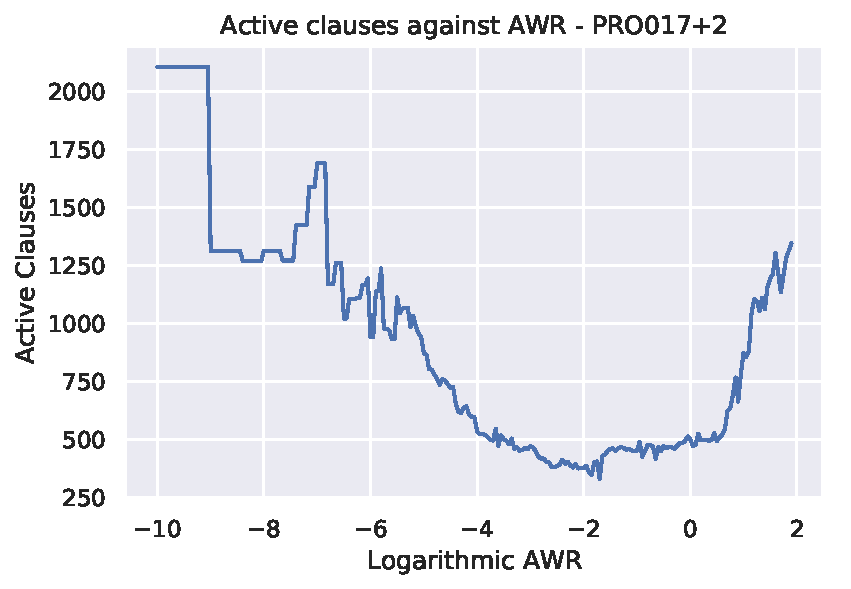
\includegraphics[width=0.8\textwidth]{example-optimal-awr}
	\caption{
The number of activations reported by Vampire after successful 1-second runs on a TPTP problem.
In between the peaks on either side, the function of \(L\) is discontinuous with large peaks and troughs, but follows an approximate trend and settles toward the global optimum.
This is typical for the observed set of problems.
}
	\label{fig:example-optimal-awr}
\end{figure}

\subsection{Experiments}
As an initial illustrative example of how varying the AWR effects the number of clauses required to be processed before a proof is found consider Figure \ref{fig:example-optimal-awr}. This shows \todo{FINISH}


  shows the effect of varying AWR on an illustrative problem from TPTP: a smaller number of activations means that fewer clauses were processed, which in general means that a proof was found faster\footnote{
It should be noted that if a small number of clauses are extremely expensive to process it may be slower than a larger number of less-expensive clauses, but in general this is a good heuristic measure for prover performance.
It also avoids reproducibility issues involved with using system timing approaches.
}.
On this problem, a good AWR value is over 400\% better by this metric than the worst AWR value.

\begin{figure}[t]
	\centering
	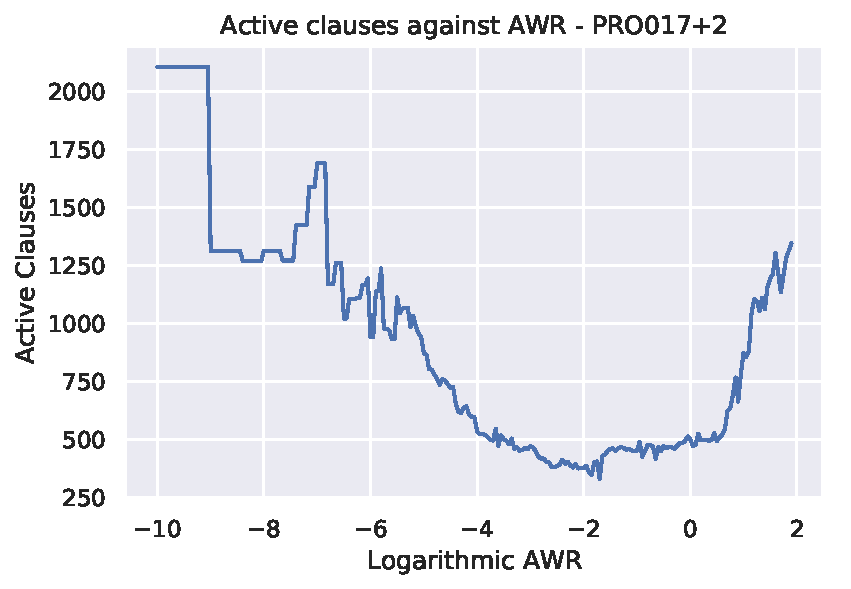
\includegraphics[width=0.8\textwidth]{example-optimal-awr}
	\caption{
The number of activations reported by Vampire after successful 1-second runs on a TPTP problem.
In between the peaks on either side, the function of \(L\) is discontinuous with large peaks and troughs, but does follow an approximate trend and settles toward the global optimum.
These properties are typical for the observed set of problems.
}
	\label{fig:example-optimal-awr}
\end{figure}

This experiment was repeated on the whole TPTP problem set, excluding problems Vampire does not support, problems which were not solved by the default mode in under a second for any AWR value, and problems solved in pre-processing.
The whole set yielded similar AWR data for 7,947 problems.
These data show that while there is no ``best'' AWR for the whole set (Table \ref{tab:no-best-awr}), choosing a good AWR value for a problem is well-rewarded (Table \ref{tab:awr-improvement}).

\noindent
 \todo{Can we also capture the solved/unsolved balance? Perhaps just say what \% of solved problems were solved using that ratio.}
\todo{This discussion should be expanded. Results need more explanation and we should summarise e.g. yes we confirmed assumptions.}\\

\begin{table}[t]
	\caption{The mean relative performance drop (in terms of activations compared to an optimal value) choosing a single AWR over an entire problem set causes. No setting is significantly ``better'' or ``worse'' than the others, but some have more variance in performance. A ratio of 1:4 produces an unusually well-behaved maximum performance drop. \sandm~found that 1:5 had a similar property, but this might be explained by differences in test environment.}
	\centering
	\begin{tabular}{l | c | c  c }
AWR & Maximum Drop & Mean Drop & (Standard Deviation)\\
\hline
8:1 & 150.67 & 1.37 & 1.98\\
5:1 & 122.22 & 1.33 & 1.64\\
4:1 & 101.44 & 1.32 & 1.42\\
3:1 & 105.00 & 1.29 & 1.41\\
2:1 & 112.67 & 1.27 & 1.45\\
3:2 & 119.89 & 1.27 & 1.51\\
5:4 & 125.00 & 1.26 & 1.55\\
1 & 133.56 & 1.26 & 1.63\\
2:3 & 147.67 & 1.28 & 1.79\\
2 & 162.67 & 1.31 & 1.97\\
3 & 190.56 & 1.37 & 2.30\\
4 & 17.41 & 1.38 & 0.67\\
5 & 133.67 & 1.44 & 1.70\\
6 & 106.44 & 1.47 & 1.46\\
7 & 104.89 & 1.49 & 1.44\\
8 & 101.33 & 1.53 & 1.45\\
10 & 101.78 & 1.60 & 1.53\\
12 & 101.67 & 1.65 & 1.62\\
14 & 103.00 & 1.70 & 1.75\\
16 & 101.33 & 1.74 & 1.76\\
20 & 100.89 & 1.82 & 1.94\\
24 & 101.33 & 1.89 & 2.08\\
28 & 99.22 & 1.96 & 2.24\\
32 & 100.00 & 1.99 & 2.36\\
40 & 98.78 & 2.09 & 2.64\\
50 & 98.78 & 2.17 & 2.88\\
64 & 101.22 & 2.28 & 3.19\\
128 & 107.44 & 2.57 & 4.16\\
1024 & 222.01 & 2.83 & 7.55
	\end{tabular}

	\label{tab:no-best-awr}
\end{table}

\begin{table}
	\caption{Relative performance gain, showing the ratio in activations between the best AWR setting for a given problem and another base setting. We compare the base settings of 1:1 (Vampire's default), 1:5 (the best-behaved from Table \ref{tab:no-best-awr}), and the worst setting for the problem.}
	\centering
	\begin{tabular}{c | c | c c}
		& Maximum Gain & Mean Gain & (Standard Deviation)\\
		\hline
		1:1 & 133.56 & 1.26 & 1.63 \\
		1:5 & 133.67 & 1.44 & 1.70 \\
		(worst) & 222.01 & 3.95 & 7.60 \\
	\end{tabular}
	\label{tab:awr-improvement}
\end{table}

%%%%%%%%%%%%%%%%%%%%%%%%%%%%%%%%%%%%%%%%%%%
\section{Variable AWR for Vampire} 

In this section we motivate and define a variable clause selection approach.

%%%%%%%
\subsection{The Optimal AWR Over Time} \label{sec:varying:study}

Although choosing a good AWR value is important, this is covered in part by the use of strategy scheduling~\cite{CADE18} in which many AWR values are tried in sequence (along with other prover options).
Additionally, given that varying the AWR can have such a large impact, it seems likely that a constant AWR fixed for the entire proof search is unlikely to be optimal for any given problem.
This can be shown by running Vampire with a randomised sequence of age/weight ratios given by a random walk repeatedly, then finding the best after a large number of repetitions.
Applying this method with 10,000 repetitions to the problem seen earlier (\texttt{PRO017+2}) yields the example AWR trend shown in Figure \ref{fig:random-walk}, which reduces the best number of activations from 330 with a fixed AWR, to 287 with a varying AWR.

Unsurprisingly, in ad-hoc experiments on other problems, the best shape is rarely constant.
This suggests that implementing other shapes, such as an increasing or decreasing trend, might lead to quicker proofs in the Vampire theorem prover.

\begin{figure}[t]
	\centering
	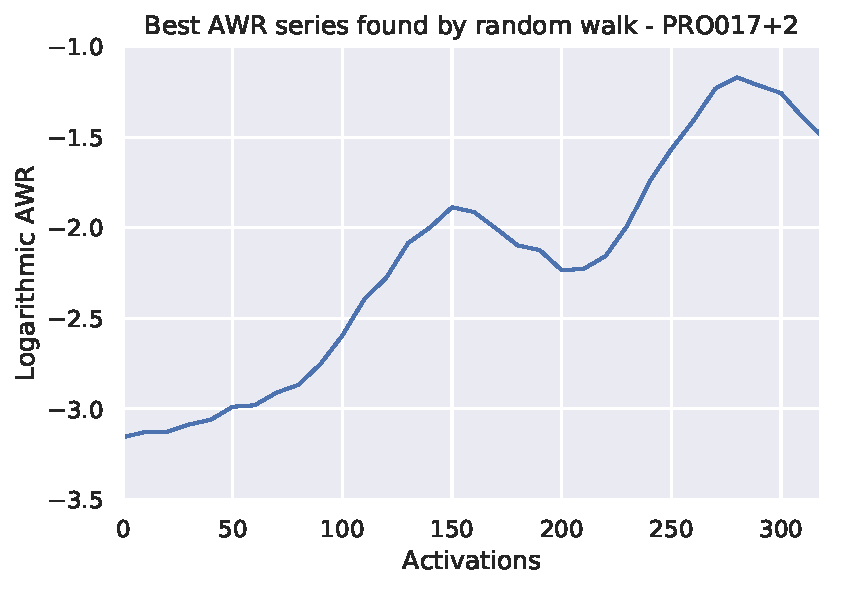
\includegraphics[width=0.8\textwidth]{random-walk}
	\caption{The AWR series that produced the lowest number of activations on a particular problem, smoothed in order to show the actual effect on proof search. This is a search strategy that a single fixed AWR cannot reproduce.}
	\label{fig:random-walk}
\end{figure}

%%%%%%%
\subsection{Varying AWR in Vampire} \label{sec:varying:implementation}

If changing AWR is sometimes useful for finding proofs more quickly, this could be useful as a Vampire option.
In general we would like to describe any possible sequence that the AWR could follow during proof search.
However, some details constrain the design space:
\begin{enumerate}
	\item Changing the AWR too frequently or sharply has little effect, due to the ``balancing'' algorithm --- see Section \ref{sec:introduction}.
	\item A general (configurable) \emph{shape} is more likely to be widely applicable than a specific series of data points.
	\item The shape must extend naturally to an indefinitely-long proof search.
\end{enumerate}

In this work we selected two general trends to explore: a trend away from the original (fixed) AWR toward 1:1 (``decay''), and a trend from 1:1 toward the original setting (``converge'').
Since a simple linear shape does not extend well to indefinite proof search (it is unclear what should happen after either 1:1 or the target AWR is reached), an exponential decay function is used instead, as shown in Figure \ref{fig:decay-and-converge}.

\todo{What are these figures showing?}

These shapes are further parameterised by an integral \emph{shape frequency} setting, which controls the rate of decay or convergence: every \(n\) steps, the difference between the current and the target AWR is halved, rounding where necessary.
In future, this might allow the use of repeating patterns such as a sinusoid, hence \emph{frequency}.

Our approach here was restricted by the balancing algorithm used internally, as AWR steps must be discrete and do not take effect immediately.
An alternative approach might use an age/weight probability, rather than a ratio, from which age or weight decisions would be pseudo-randomly (but reproducibly) taken with the use of a seeded PRNG.
This would permit use of continuous age/weight functions, but would also introduce the possibility of ``getting unlucky'' in which a clause preferred by the age/weight probability is not selected due to an improbable-but-possible series of PRNG samples.

\begin{figure}
	\subfloat{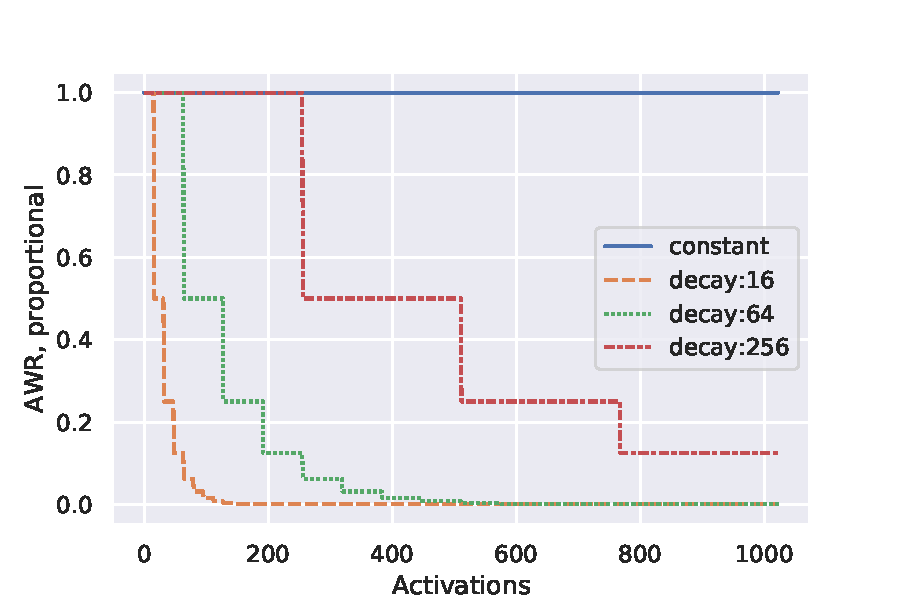
\includegraphics[width=0.5\textwidth]{shape-decay}}
	\subfloat{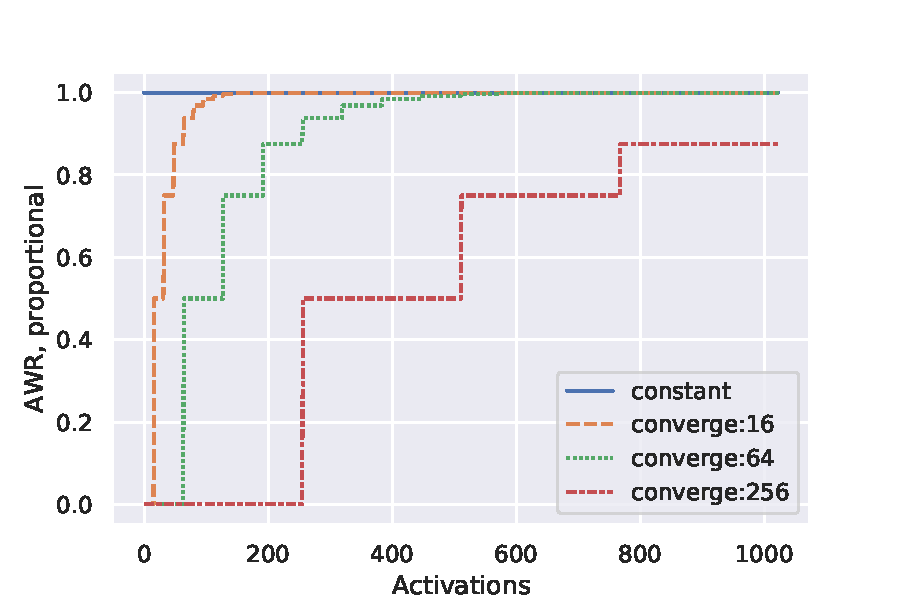
\includegraphics[width=0.5\textwidth]{shape-converge}}
	\caption{The new \emph{decay} and \emph{converge} AWR shapes as implemented in Vampire. Different curves exhibit the effect of the AWR shape frequency setting.}
	\label{fig:decay-and-converge}
\end{figure}

Together, these new settings allow a number of new option combinations, which can be used in conjunction with Vampire's portfolio mode pending integration into the strategy schedules.
This version of the prover is currently in a separate branch in the main Vampire source repository\footnote{\texttt{https://github.com/vprover/vampire/tree/awr-shapes}}.

%%%%%%%%%%%%%%%%%%%%%%%%%%%%%%%%%%%%%%%%%%%
\section{Experimental Evaluation}
\label{sec:experiments}

\todo{Change marketing here. Success is adding new options to portfolio mode. Only mention CASC once and refer to portfolio mode elsewhere.}

In practice, decaying from an age-biased initial AWR to 1:1 (or converging backwards) was not found to be an improvement.
However, age/weight shapes decaying from or converging to a weight-based AWR were found to be useful in some cases.
An experimental evaluation of this approach on the TPTP~\cite{tptp} benchmark follows.

Vampire first ran to establish baseline performance in its competition \emph{CASC mode} on all problems in TPTP, with a wallclock time limit of 300 seconds.
For experimental purposes, the same environment was preserved with the exception of activating the new ``shapes'' settings with a range of different shape frequencies.
The baseline solved 13,057 problems in total.
No experimental configuration improved on this figure, but some problems not solved by baseline were solved by the new configurations, and some entirely new problems were solved.

\subsection{Benchmark Performance}
Figure \ref{tab:results} shows the performance in terms of solved problems of all the configurations tested.
These data show that configurations which are more similar to the baseline (i.e. slow decay or fast convergence) achieve more similar performance, as expected.
In total, 134 problems were solved by the new configurations that were not solved by the baseline.

\begin{table}
	\caption{
Results for the tested configurations.
\emph{Proved} refers to the total number of problems a configuration solved.
\emph{Fresh} is the number of problems a configuration solved which were not solved by the baseline.
\emph{Uniques} is the number of problems a configuration solved which were not solved by any other configuration.
\emph{\(u\)-score} is a refined unique score which correlates to a configuration's utility in solving new problems, as used in Hoder \emph{et al.}~\cite{u-score}.
	}
	\centering
	\begin{tabular}{l l l l l l}
		Configuration & Frequency & Proved & Fresh & Uniques & \(u\)-score\\
		\hline
		baseline & -- & 13057 & 0 & 1 & 714.2\\
		converge & 1 & 13039 & 24 & 3 & 714.3\\
		converge & 5 & 13029 & 27 & 1 & 709.5\\
		converge & 10 & 13028 & 35 & 5 & 714.3\\
		converge & 50 & 13015 & 45 & 5 & 712.8\\
		converge & 100 & 12976 & 51 & 1 & 705.9\\
		converge & 500 & 12895 & 63 & 4 & 698.3\\
		converge & 1000 & 12837 & 52 & 0 & 688.6\\
		converge & 5000 & 12775 & 53 & 1 & 682.4\\
		converge & 10000 & 12751 & 53 & 0 & 678.7\\
		decay & 1 & 12698 & 48 & 1 & 673.6\\
		decay & 5 & 12702 & 51 & 1 & 674.9\\
		decay & 10 & 12698 & 48 & 1 & 674.2\\
		decay & 50 & 12712 & 49 & 2 & 679.1\\
		decay & 100 & 12726 & 46 & 1 & 678.8\\
		decay & 500 & 12795 & 29 & 1 & 685.5\\
		decay & 1000 & 12860 & 29 & 2 & 692.6\\
		decay & 5000 & 12982 & 16 & 2 & 707.1\\
		decay & 10000 & 13002 & 7 & 0 & 706.3\\
		\hline
		converge & (combined) & 13167 & 117 & -- & --\\
		decay & (combined) & 13106 & 93 & -- & --\\
	\end{tabular}
	\label{tab:results}
\end{table}

\subsection{New Problems}
Some problems were solved which were marked as ``Unknown'' status in the TPTP headers.
Vampire baseline (and several configurations) were able to solve \texttt{GEO120+1}, but only converging with frequency 50 solved \texttt{SET345-6} and only decaying with frequency 1 solved \texttt{LAT320+3}.


%%%%%%%%%%%%%%%%%%%%%%%%%%%%%%%%%%%%%%%%%%%
\section{Conclusions and Future Work}
\label{sec:conclusions}

\todo[inline]{this is a thing, you can do it, you should do it (?), we can probably do better}
\todo[inline]{more shapes, better ways of doing frequency decay, integrate into existing strategy schedules}

\bibliographystyle{plain}
\bibliography{references}
\end{document}
